\documentclass{article}[10pt]
\usepackage{longtable}
\usepackage{lscape}
\usepackage{booktabs}
\newcommand{\specialcell}[2][c]{%
  \begin{tabular}[#1]{@{}l@{}}#2\end{tabular}}
	% \specialcell{Date,\\duration}
\usepackage{rotating, multirow}
\usepackage[flushleft]{threeparttable}
\usepackage{graphicx}% http://ctan.org/pkg/graphicx
	
\begin{document}


	\begin{table}[h]
		  \begin{threeparttable}
	\begin{tabular}{@{}lllllllll@{}}	
	\toprule
	ID  & Date        & Participants      & Prototypes tested \\
	\midrule
	G1  & Apr. 2012  & 9 filed workers     & W1, D1 \\
	G2  & May 2012   & 1 disaster manager  & C1, W1 \\
	G3  & Jul. 2013  & 3 field workers, 1 manager & D2 \\
	G4  & Sept. 2013 & 8 IT students, 4 HCI experts & D2 \\
	\bottomrule
	\end{tabular}
	\begin{tablenotes}
	     \item
	    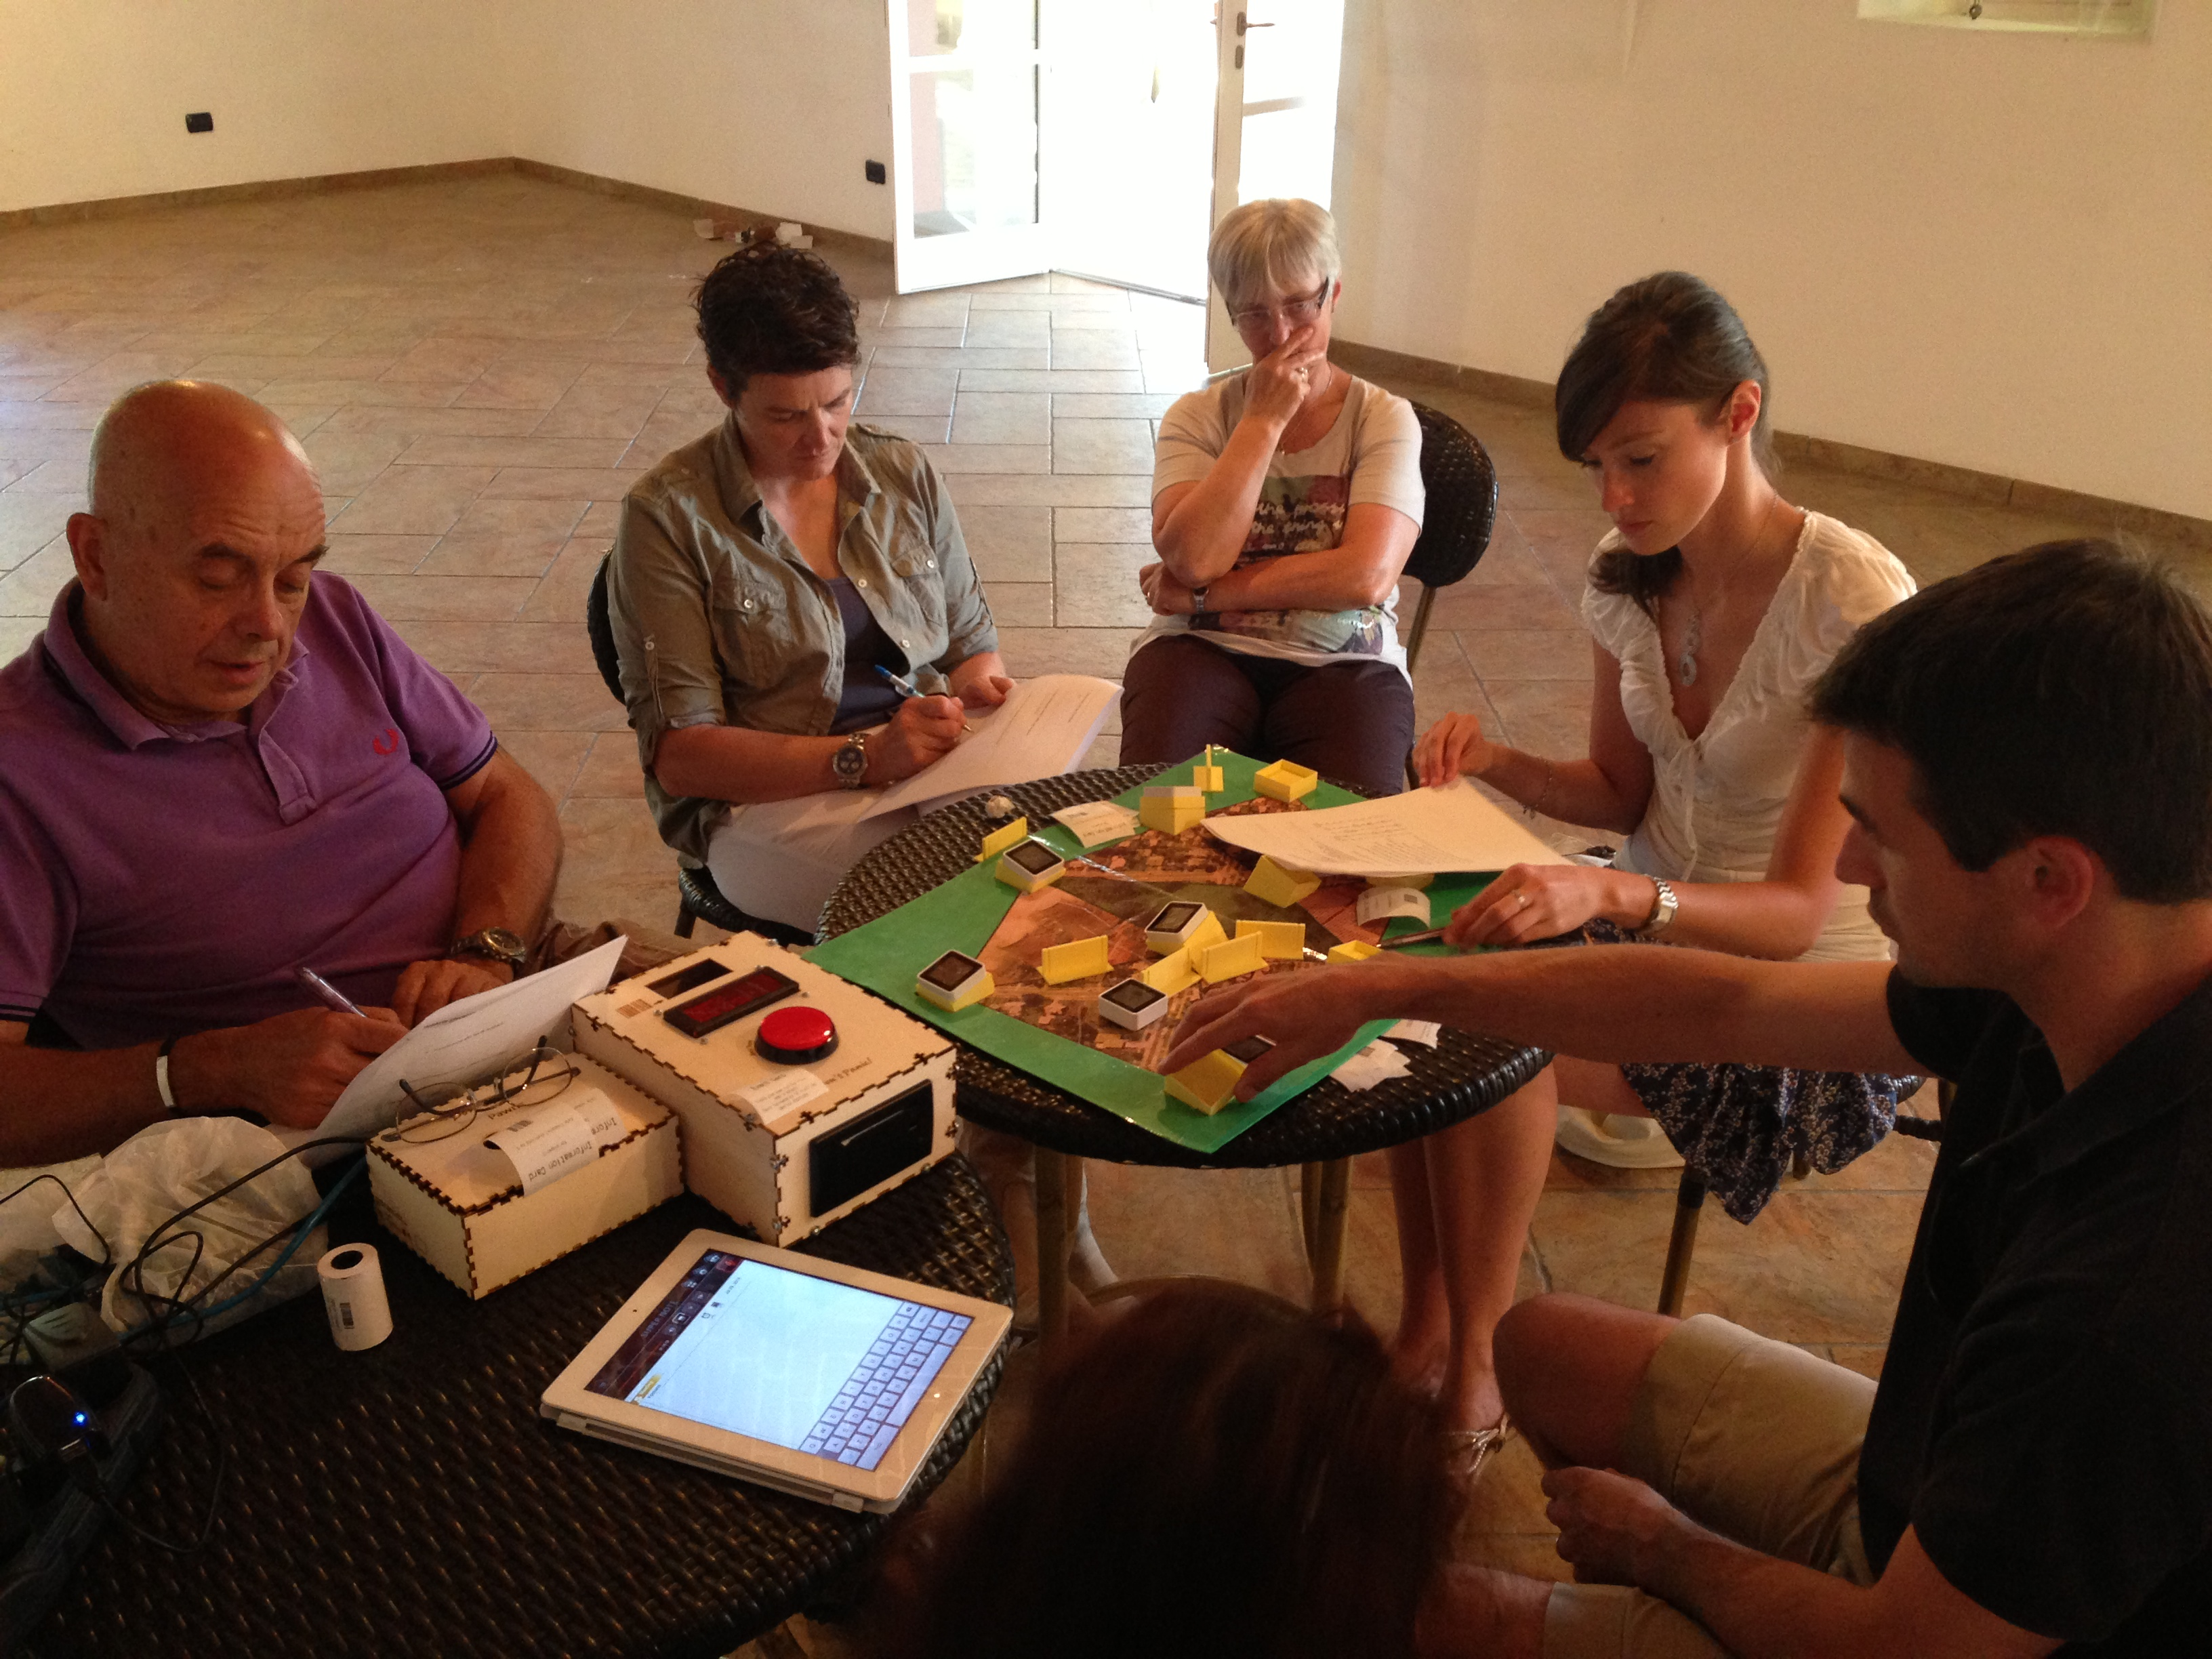
\includegraphics[width=\linewidth]{d2_prototype}
	   \end{tablenotes}
	 \end{threeparttable}
	\caption{Description of focus groups performed  Workers busy testing D2 prototype and filling in USU questionnaires}
	\label{prototypes}
	\end{table}




\begin{table}[h]
\begin{tabular}{@{}lllllllll@{}}	
%\begin{tabular}{@{}p{0.3cm}p{3cm}p{0.3cm}p{0.3cm}p{3cm}p{0.25cm}p{0.25cm}p{0.25cm}p{1.5cm}}
\toprule
   &                             & \multicolumn{2}{c}{Aim}                    &          & \multicolumn{3}{c}{Methods}            &    \\ \cline{3-4} \cline{6-8}  \noalign{\smallskip}
ID & Date, duration & \begin{turn}{90}Exploratory\end{turn} & \begin{turn}{90}Evaluation\end{turn} & Participants & \begin{turn}{90}Observations\end{turn} & \begin{turn}{90}Interviews\end{turn} & \begin{turn}{90}Questionnaires\end{turn}   & Papers \\ \midrule \noalign{\smallskip}

F1  & Mar. 2011, 2 days            & \textbullet &   & several teams                & \textbullet                          & \textbullet                         &                                         &  P1   \\
F2  & Oct. 2011, 3 days            & \textbullet & & \specialcell[t]{several teams,\\1 manager}      & \textbullet                          & \textbullet                         &                                          & P1, P3        \\
F3  & Oct. 2012, 2 days            & \textbullet & \textbullet & \specialcell[t]{5 field workers,\\1 manager}   & \textbullet                          & \textbullet                         &                                          &  P1, P3  \\ 
F4  & Apr. 2013, 3 days            & \textbullet & \textbullet & \specialcell[t]{4 field workers,\\1 manager}   & \textbullet                          & \textbullet                         & \textbullet                              & P1, P3, P2   \\
F5*  & Dec. 2013, 30 days          & & \textbullet & 8 field workers              &                                      &                                     & \textbullet                               & P2, P3, P6    \\
F6  & Apr. 2014, 2 days            & & \textbullet & \specialcell[t]{27 field workers,\\1 manager} & \textbullet                          &                                     & \textbullet                               &  P2, P3, P6   \\ \noalign{\smallskip} \hline \noalign{\smallskip}
\multicolumn{9}{l}{*The author was not present during the study} \\ \bottomrule
\end{tabular}
\caption{Description of field studies performed}
\label{field-studies}
\end{table}


\begin{table}[h]
	  \begin{threeparttable}
\begin{tabular}{@{}lllllllll@{}}	
	\toprule
	       &               &               &                         & \multicolumn{3}{c}{Development}      &           &              \\ \cline{5-7}  \noalign{\smallskip}
	\specialcell[b]{ID\\Ver.}     & Name           & Released     & Prototyping tools  & \begin{turn}{90}Software\end{turn} & \begin{turn}{90}Hardware\end{turn} & \begin{turn}{90}Construction\end{turn}   & Papers     & \specialcell[b]{Field\\studies} \\
	\midrule \noalign{\smallskip}
    C1     & CroMAR         & Jul. 2011    & iOS,    & \textbullet &       &                & P1,P2      & F1,F2 \\
    C2     &                 & Jul. 2012    & Augmented Reality                        & \textbullet &           &              & P2        & F3, F4 \\
	\hline \noalign{\smallskip}
	W1     & WATCHiT         & Jan. 2012    & Arduino, Textiles         & \textbullet & \textbullet &          & P3         & F2 \\
    W2     &                 & Aug. 2012    & ZigBee, Bluetooth           & \textbullet & \textbullet &          & P3         & F2 \\
    W3     &                 & Sept. 2012   &          & \textbullet  & \textbullet &          & P3         & F3, F4 \\
    W4     &                 & Aug. 2013    &            & \textbullet & \textbullet & \textbullet  & P2, P3   & F5, F6 \\
    \hline \noalign{\smallskip}
    D1     & Don't Panic     & Mar. 2013    & Paper, wood     & & & \textbullet  & P4, P5   & F1 \\
    D2     &                 & Aug. 2013    & \specialcell[t]{Sifteo, RapsberryPi\\Laser cut}  & \textbullet & \textbullet & \textbullet & P5 & F1 \\
	\bottomrule
\end{tabular}
\begin{tablenotes}
     \item
    \includegraphics[width=\linewidth]{prototypes}
   \end{tablenotes}
 \end{threeparttable}
\caption{Description of prototypes implemented}
\label{prototypes}
\end{table}




\begin{landscape}
\begin{longtable}{p{2cm}p{3cm}p{3cm}p{3cm}p{4cm}p{1cm}p{1cm}}
ID(*=key study) & Date, duration   & Setting  & Participants  & Research Methods \newline Research Activity & RQs & Research Papers \\ 
\hline
1(*)   & March 2011, 2 days     & Real work   & several teams    & Observations, interviews User study.  & 2   & P1  \\
2(*) & October 2011, 3 days   & Simulated work in a maxi emergency & several teams, 1 manager     & Observations, interviews, video analysis. Formative evaluation of CroMAR v01. & 2   & P1 \\
3  & April 2012, 1 day      & Focus group    & 9 field workers, 1 manager   & Interviews. Evaluation of WATCHiT v01 and Don't Panic paper mockup. & 1-2 & P3-P5     \\
4  & May 2012, 1 day        & Focus group      & 1 manager     & Observation, Interview. Formative evaluation of WATCHiT v02 and CroMAR v02  & 1-2 & P1-P3           \\
5(*) & October 2012, 2 days   & Simulated work    & 5 field workers, 1 manager   & Observation, interviews, video analysis. Formative Evaluation of WATCHiT v03 and CroMAR v02  & 1-2 & P1-P3   \\
6   & April 2013, 3 days     & Simulated work in a maxi emergency & 4 field workers, 1 manager   & Observation, interviews, video analysis, questionnaires. Summative evaluation of CroMAR v02, formative evaluation of WATCHiT v03 & 1-2 & P1-P3    \\
7(*) & July 2013, 1 day       & Focus group    & 3 field workers, 1 manager   & Observations, interviews, video analysis, questionnaires. Formative evaluation of Don't Panic v01  & 2   & P4              \\
8      & September 2013, 1 day  & Focus group    & 8 IT students, 4 HCI experts & Observations, interviews, video analysis, questionnaires. Formative evaluation of Don't Panic v01    & 2   & P4     \\
9     & December 2013, 30 days & Simulated work      & 8 field workers      & Questionnaires Summative evaluation of WATCHiT v04      & 1   & P2-P3-P7        \\
10(*)  & April 2014, 2 days     & Simulated work       & 27 field workers, 1 manager  & Observations, Questionnaires Summative evaluation of WATCHiT v04    & 1   & P2-P3-P7  \\ 
\end{longtable}
\end{landscape}


\end{document}